\documentclass[aspectratio=169, 11pt]{beamer}
\usetheme{default}
\useinnertheme{circles}
\usepackage[T1]{fontenc}
\usepackage{lmodern}
\usepackage{tikz}

% Your colour set. Change the hex codes to restyle every slide.
\definecolor{slate}{HTML}{2E3440}
\definecolor{mist}{HTML}{ECEFF4}
\definecolor{teal}{HTML}{3B8B8B}
\definecolor{soft}{HTML}{8A94A6}

\setbeamercolor{normal text}{fg=slate, bg=white}
\setbeamercolor{structure}{fg=teal}
\setbeamercolor{frametitle}{fg=slate}
\setbeamercolor{title}{fg=slate}
\setbeamercolor{subtitle}{fg=teal}
\setbeamercolor{author}{fg=soft}
\setbeamercolor{date}{fg=soft}
\setbeamercolor{block title}{fg=teal, bg=mist}
\setbeamercolor{block body}{fg=slate, bg=mist}
\setbeamercolor{footline}{fg=soft}

\setbeamerfont{frametitle}{size=\Large, series=\bfseries}
\setbeamerfont{title}{size=\huge, series=\bfseries}
\setbeamertemplate{navigation symbols}{}
\setbeamertemplate{blocks}[rounded]
\setbeamertemplate{title page}{
  \vspace{2.5cm}
  {\usebeamerfont{title}\usebeamercolor[fg]{title}\inserttitle\par}
  \vspace{0.4em}
  {\large\usebeamercolor[fg]{subtitle}\insertsubtitle\par}
  \vspace{2em}
  {\usebeamercolor[fg]{author}\insertauthor\quad\usebeamercolor[fg]{date}\insertdate\par}
}
\setbeamertemplate{footline}{
  \usebeamercolor[fg]{footline}\hspace{1.2em}\scriptsize\insertshorttitle\hfill\insertframenumber\hspace{1.2em}\vspace{0.8em}
}

% Edit the title, subtitle, author and date.
\title[Quiet Slides]{Quiet Slides}
\subtitle{A calm starting point for any talk}
\author{Your Name}
\date{September 2026}

\begin{document}

\begin{frame}[plain]
  \titlepage
\end{frame}

\begin{frame}{One idea per slide}
  \begin{itemize}
    \item Keep a single message on each slide.
    \item Use short phrases, not paragraphs.
    \item Let white space do the work.
  \end{itemize}
\end{frame}

\begin{frame}{Two columns}
  \begin{columns}[T]
    \begin{column}{0.46\textwidth}
      \begin{block}{Before}
        Dense slides that people read instead of listening.
      \end{block}
    \end{column}
    \begin{column}{0.46\textwidth}
      \begin{block}{After}
        Short statements that support what you say.
      \end{block}
    \end{column}
  \end{columns}
\end{frame}

\begin{frame}{A simple figure}
  \centering
  % Edit the heights (second number) to change the bars.
  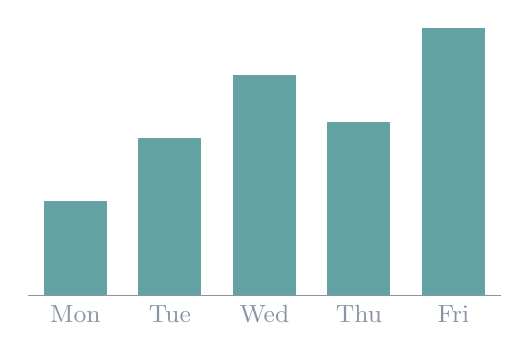
\begin{tikzpicture}
    \foreach \x/\h/\lab in {0/1.2/Mon, 1.2/2.0/Tue, 2.4/2.8/Wed, 3.6/2.2/Thu, 4.8/3.4/Fri} {
      \fill[teal!80] (\x,0) rectangle ++(0.8,\h);
      \node[below, text=soft, font=\small] at (\x+0.4,0) {\lab};
    }
    \draw[soft] (-0.2,0) -- (5.8,0);
  \end{tikzpicture}
\end{frame}

{
\setbeamercolor{background canvas}{bg=slate}
\begin{frame}[plain]
  \centering\vfill
  {\Huge\bfseries\textcolor{white}{A statement slide}}\\[0.6em]
  {\large\textcolor{teal!60}{for the one sentence people should remember}}
  \vfill
\end{frame}
}

\begin{frame}{Numbered steps}
  \begin{enumerate}
    \item Outline the story first.
    \item Draft slide titles as full sentences.
    \item Fill in only what each title needs.
  \end{enumerate}
\end{frame}

\begin{frame}[plain]
  \centering\vfill
  {\Huge\bfseries Thank you}\\[0.8em]
  {\textcolor{soft}{you@example.org}}
  \vfill
\end{frame}

\end{document}
